\documentclass[./Thesis]{subfiles}


\graphicspath{{./Images/}}



\begin{document}
\chapter{Straw Tube Tracker Systematics}

With the straw tube trackers being an important part to a variety of measurement that need to be made it is important that the systematic uncertainties of the system are investigated and understood.  The measurements that are being made by the trackers are pitch correction, beam dynamics, electric field corrections, along with the electric dipole moments measurement.  This chapter will explain specifically the errors of cross talk and hit resolution in the straw detectors and how these errors were characterized and their relative effect on the measurements.

\section{Cross Talk in the Straw Trackers}

Cross Talk is an effect when there is a particle signal in one wire which causes a signal in another wire.  This could be catastrophic for the measurement especially in the pitch correction and the EDM measurement as this would throw off the extrapolated y position due to the bias in the track fitting.  Furthermore, If I add in another hit in a straw when there is not supposed to be a hit then this could shift the particular momentum at a plane and cause an error in the fit or an extra deviation in the fitting algorithm.  Refer to Fig.\ref{fig:PicXtalk}, if a digit that occurs at position 1 and 2 this could show that the particle trajectory in the right direction. Alternatively, if a digit occurs in position 2 and 3 this would show the particle trajectory would be moving to the left direction throwing of the results at this plane.  This section will explain the process how I characterized and added this effect into simulation to see how much of an effect this will cause on the extrapolation y positions and radial positions in the detector.

\begin{figure}
	\centerline{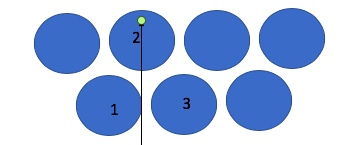
\includegraphics[height=50mm]{CrossTalkEval.jpeg}}
	\caption[ Pictorial Representation of Picking out Cross Talk]{ A pictorial representation of how Cross Talk was picked out}
	\label{fig:PicXtalk}
\end{figure}


\subsection{General Explanation of Cross Talk}

	Cross talk, or what we are calling cross talk, in the detectors could be caused by multiple different processes.  Firstly, because the aluminized drift tubes are conductive and these tubes are neighboring each other this create a capacitive coupling between straws, therefore allowing charge to exchange between the wires.  The next source of cross talk in the detector could be from within the electronic boards themselves.  When traces on a printed circuit boards are neighboring this creates an inductive or capacitive couple between the traces causing a signal from one trace to bleed into another trace.  It is unknown which of these are the greatest effect, but they should have similar properties, and this is what we would consider cross talk in the detectors.  Thirdly, although not technically cross talk we could have a case when there is a muon in the detectors, and it decays to a positron therefore causing a signal in another wire and confusing the tracking results.  In addition, we could radiative effects coming from the positrons also creating neighboring hits.  All these properties are lumped together in this analysis since it is only needed to evaluate the properties of these effects and add it into simulation to observe these effects on the tracking analysis.
	
\subsection{Evaluation of the properties of Cross Talk}

	In order to add the effects of cross talk into the simulation and to understand the true effects that cross talk has on our track finding and fitting we needed to ask the questions when does cross talk occur after the first digit, is there any correlations between the data products of the cross talk hit or the primary hit (The hit that causes the cross talk), how much cross talk occurs in our detectors...etc. To do this it is necessary to establish the know properties of cross talk just from the very definition of it being cross talk. Firstly, we know that cross talk is caused by something else so it has to occur after another hit in the detector. Secondly, we know that from the sources of cross talk established earlier we are most likely going to find cross talk in the neighboring wire. Lastly, since the cross talk signal again is caused by charge in another wire the primary signal charge cannot be larger than the cross talk signal charge.  These properties will be important for selecting out particular tracks and will allow us to pick out cross talk signals.
	
	Firstly, it was necessary to get a known cross talk sample.  To get these known cross talk signals we looked at a case where there is only one particle that was going through the detector at a time.  The next criterion that was necessary is that we required there to be two hits in the same layer of the detector without any hits being in the opposing layer.  To take out the case of decaying muons in the detector there is a momentum cut at 2300MeV.  Now there is only the case where there is a primary digit and a cross talk digit, with the primary digit occurring first in time.  The time distribution between the primary digit and the cross talk digit is found in Fig.\ref{fig:TimeXtalk}, which has an odd shape mainly due to the fact that there are multiple different situations of cross talk occurring. Next, if we look at the drift time distribution for cross talk, found in Fig.\ref{fig:DriftXtalk}, it is shown that generally the drift time for cross talk is fairly large. Furthermore, looking at the distance of closest approach distribution of cross talk in Fig.\ref{fig:DCAXtalk} , due to the large drift time, results in most of the cross talk looking like a particle hit on the edge of the wire.
		
\begin{figure}
	\centerline{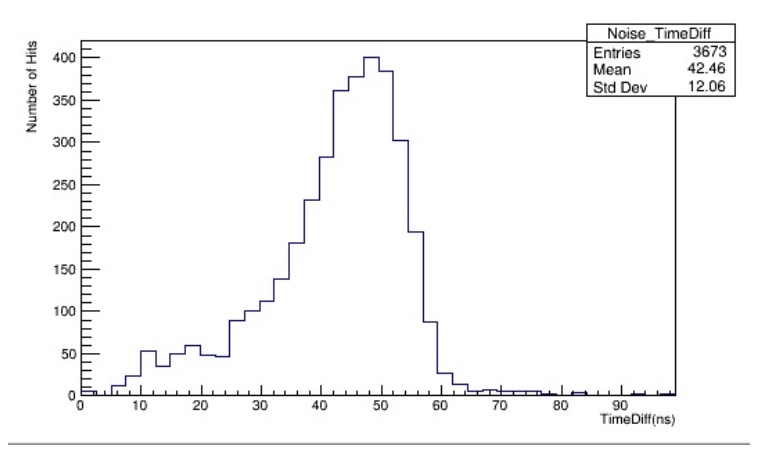
\includegraphics[height=95mm]{TimeDiffXtalk.jpeg}}
	\caption[ Cross Talk Time Distribution]{ The observed cross talk time difference distribution from data at 1550V.}
	\label{fig:TimeXtalk}
\end{figure}

\begin{figure}
	\centerline{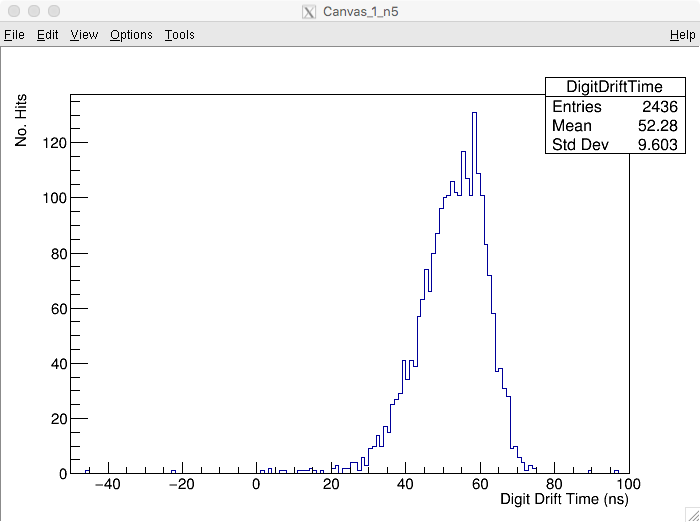
\includegraphics[height=95mm]{DriftTimeXtalk.png}}
	\caption[ DriftTime Distribution of Cross Talk]{ The observed cross talk drift time distribution from data at 1550V.}
	\label{fig:DriftXtalk}
\end{figure}
	
\begin{figure}
	\centerline{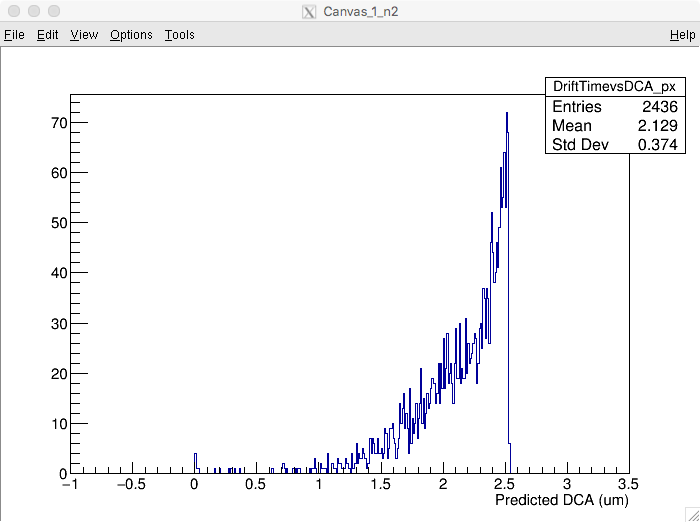
\includegraphics[height=95mm]{DCAXtalk.png}}
	\caption[ Distance of Closest Approach Distribution of Cross Talk]{ The observed distance of closest approach distribution from data at 1550V.}
	\label{fig:DCAXtalk}
\end{figure}
	
	In order to add the effects of cross talk into the simulation and to understand the true effects that cross talk has on our track finding and fitting we needed to ask the questions when does cross talk occur after the first digit, is there any correlations between the data products of the cross talk hit or the primary hit (The hit that causes the cross talk), how much cross talk occurs in our detectors...etc. To do this it is necessary to show the known properties of cross talk just from the very definition of it being cross talk. 

 Firstly, we know that cross talk is caused by something else, therefore it must occur after another hit in the detector.  Secondly, we know that from the sources of cross talk we are most likely going to find cross talk in the neighboring wire.  Lastly, since the cross-talk signal again is caused by charge in another wire the primary signal charge cannot be larger than the cross-talk signal charge.  These properties will be important for selecting the tracks and will allow us to pick out cross talk signals.
	
	Next it was necessary to evaluate the general properties of cross talk, they are not necessarily important for the simulation; However, it is nice to know and document the properties as a quality control standard.  In addition, this gives a good double check that the method to select the cross-talk digits are valid.  It was found that the hit width distribution, explained previously, had an odd shape with one little hump on the small hit width side and a large overlaying hump as shown in Fig. \ref{fig:hitWidth}. It seems that this would be the cross talk since we would expect the cross-talk signal to be small, at least smaller than the primary digit.  To prove this, the earlier method to select out cross talk and the primaries method was used.  Putting these into the hit width distribution Fig. \ref{fig:hitWidthAll} it is found that the assumption that digits that are larger are more likely to cause cross talk digits that are small is valid.
	
\begin{figure}
	\centerline{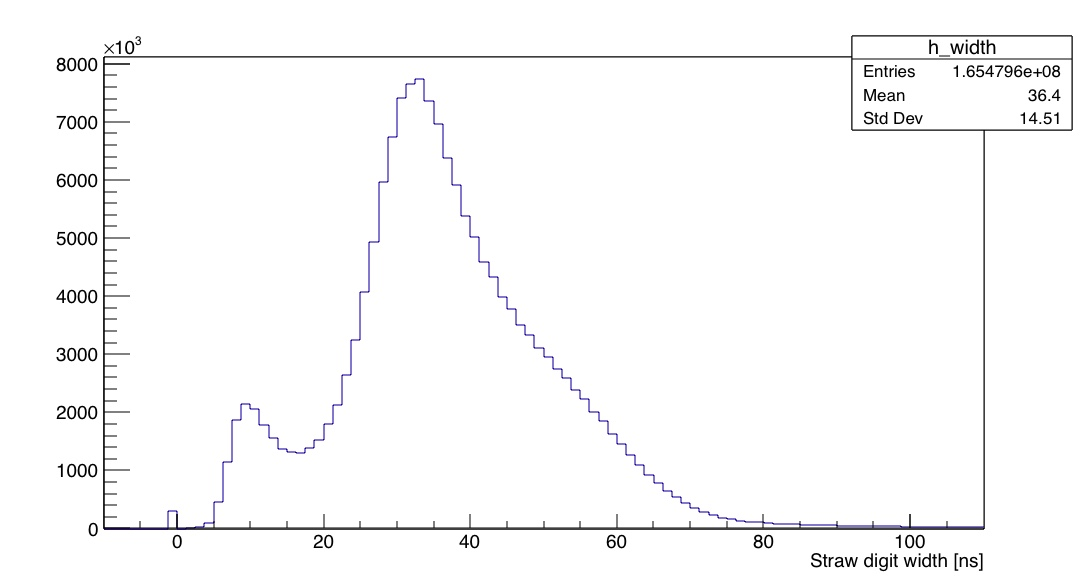
\includegraphics[height=95mm]{NormalHitWidth.jpeg}}
	\caption[ HitWidth]{ The Normal Hit width distribution without track selection}
	\label{fig:hitWidth}
\end{figure}


\begin{figure}
	\centerline{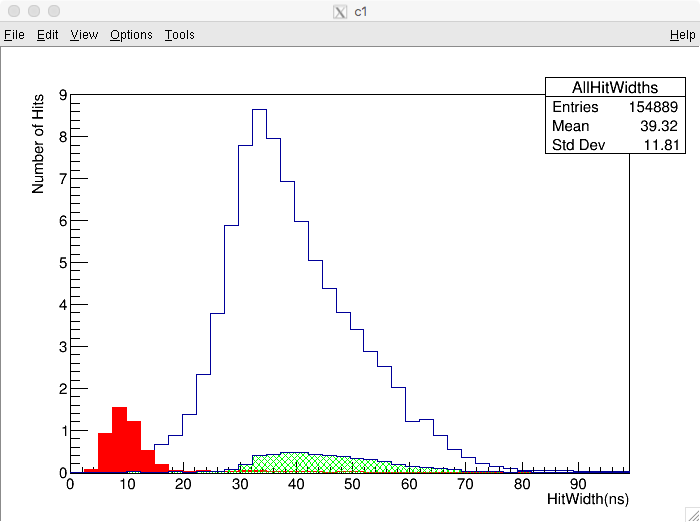
\includegraphics[height=95mm]{HitWidthsXtalkComparison.png}}
	\caption[ HitWidth with cross talk and primary digits]{ The Normal Hit width distribution overlaid with primary digits }
	\label{fig:hitWidthAll}
\end{figure}

	
	
	The cross talk in the detector should be dependent on the gain in the straws and therefore the cross talk will be dependent on external weather effects due to the properties of the argon ethane gas changing.  To investigate this, a data set which was ran over 60 hours was used.  Then the average temperatures and pressures over the series of runs was observed and the number of cross talk digits versus the number of tracks found in that layer. Fig.\ref{fig:NoiseTemp} shows how the cross talk increases as a function of temperature and Fig.\ref{fig:NoisePress} shows how the cross talk I selected decreases as a function of pressure. These results are consistent with what I would expect with cross talk.  In Fig.\ref{fig:NoiseRun} shows how the cross talk varied over multiple detectors over that same 60 hour period which shows that there is a fairly large variance in cross talk from run to run. Note, the percentage on the y-axis is arbitrary since it?s the percentage of tracks, the point of these is to confirm that the properties of the digits that were collected as cross talk have the properties of cross talk.  As another double check, the gain is also dependent on the voltage on the trackers.  Therefore, we should expect that the cross talk versus voltage should give an exponential curve until we get to saturation.  In Fig.\ref{fig:plateau} shows how the gain is dependent on the voltage. Using data from different voltages in the detectors it is found that this is true given in Fig.\ref{fig:NoiseVolts}.	
	
	
\begin{figure}
	\centerline{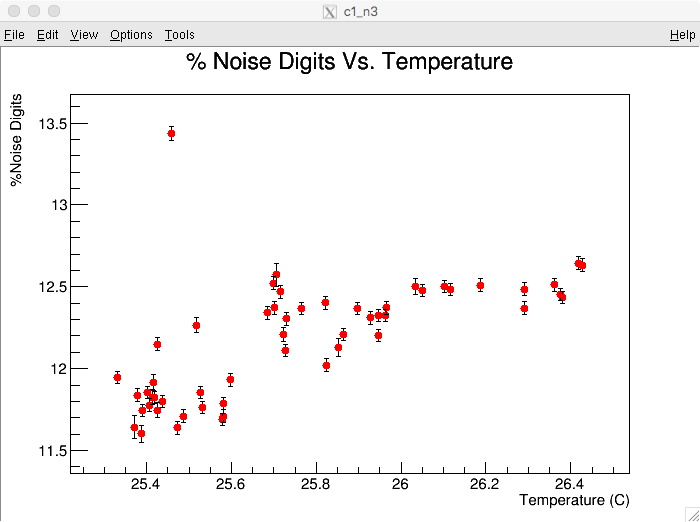
\includegraphics[height=95mm]{NoisDigjtsVsTemp.png}}
	\caption[ Cross Talk Vs. Temperature]{ The observed correlation between cross talk and temperature. Note: Not true cross talk probability.}
	\label{fig:NoiseTemp}
\end{figure}

\begin{figure}
	\centerline{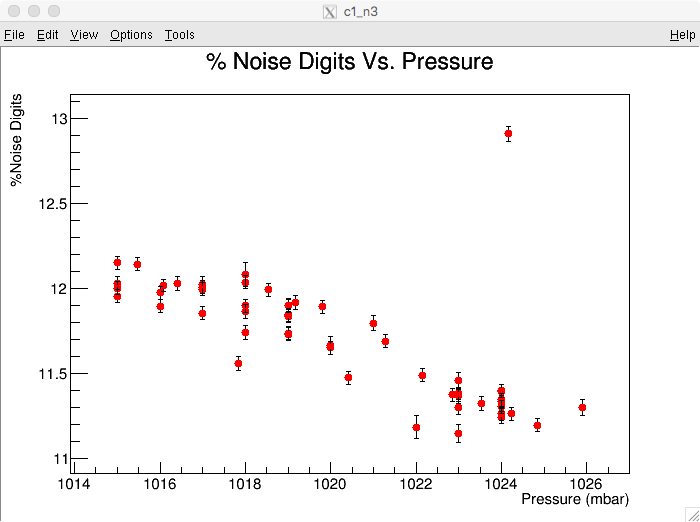
\includegraphics[height=95mm]{NoiseVsPressure.png}}
	\caption[ Cross Talk Vs. Pressure ]{ The observed correlation between cross talk and Pressure. Note: Not true cross talk probability.}
	\label{fig:NoisePress}
\end{figure}

\begin{figure}
	\centerline{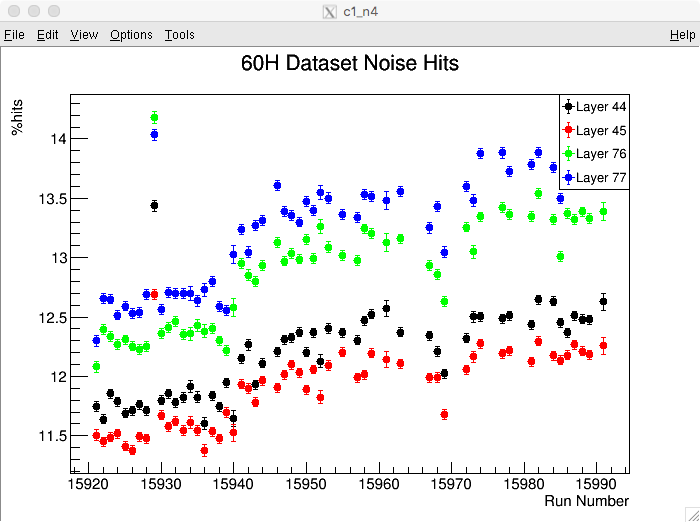
\includegraphics[height=95mm]{Noise60hDataSet.png}}
	\caption[ Cross Talk Vs. RunNumber ]{ The observed correlation between cross talk over the course of time. Note: Not true cross talk probability.}
	\label{fig:NoiseRun}
\end{figure}

\begin{figure}
	\centerline{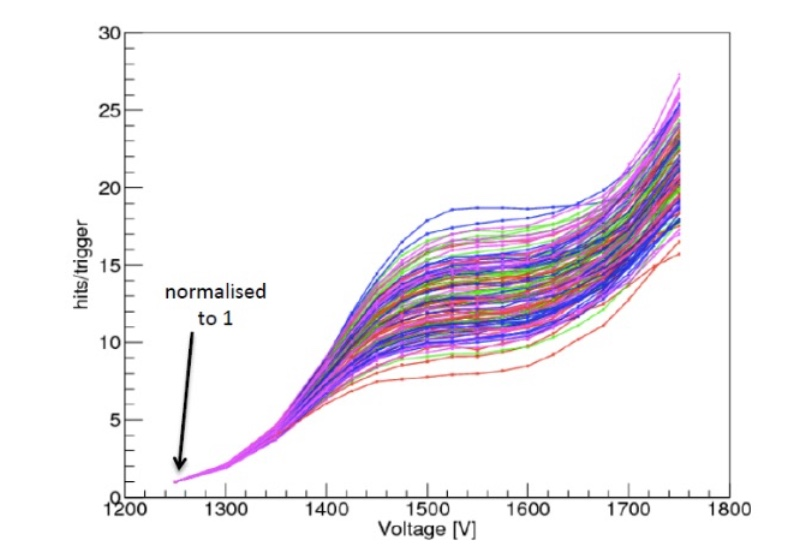
\includegraphics[height=95mm]{PlateauCurve.jpeg}}
	\caption[Plateau Plot ]{ The plateau plot of $32$ straws in the straw tracker. Y axis is essentially proportional to current in detector.}
	\label{fig:plateau}
\end{figure}


\begin{figure}
	\centerline{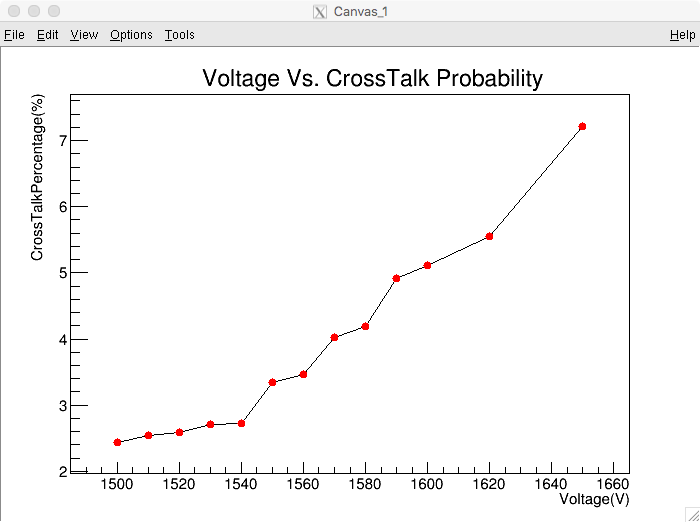
\includegraphics[height=95mm]{VoltageVsCrossTalkProbabilityMod3Stat1.png}}
	\caption[ Cross Talk Vs. Voltage (V)]{ The observed correlation between cross talk with voltage. Note: Not true cross talk probability.}
	\label{fig:NoiseVolts}
\end{figure}

	
	
\subsection{Introduction of Cross Talk into Simulation}

	Now that the properties of known cross talk signals are characterized it is now necessary to add the cross talk into a simulation to observe the effects that the cross talk has on the tracking. Firstly, it is necessary to establish at which step in the code that it is required to add in cross-talk and what properties are required so that we can randomly add this into the data. 
	
	To explain the reasoning behind this step it is necessary to explain a little bit about how the simulation that is being used works and what is being added in for data along the way.  The simulation that we used is what is called a gas gun simulation where particles are randomly positioned in the ring at their decay points with some initial momentum defined by the simulation. The particle then decays to anywhere in the ring and then we can look at the decays that hit the detectors.  The next step then picks out the specific straws that are hit and the distance from the center of the straw and then creates the digits.  These digits only have the properties of what is called the wire id, which just labels the specific straw that is hit, and the time at which the wire was hit.  Then the tracking algorithm uses this data to do the normal tracking algorithm that is shown in earlier sections.  With it was found that the best place to add in the effect of cross talk is just after the digits for the actual track are being added.  The only properties that are needed is that of those digits, such as where the cross-talk digits will occur and at what time the digits will occur. 
	
	To add the effect of cross talk into the simulation there was randomly picked some digits according to a defined percentage which is defined as a variable in my code.  Then added in is another digit into the neighboring wire to the random time distribution that was found Fig.\ref{fig:TimeDiffSim}. Next, there was regenerated all the digits along with the cross-talk digits and it was passed on to the tracking algorithm defined in earlier sections.

  To confirm that the coding was correct it is satisfactory to compare the time distribution as given in the simulation, Fig.\ref{fig:TimeDiffSim}, and the observed time distribution Fig.\ref{fig:TimeXtalk}, since this is the only defined parameter in the code. This shows that the data and the mathematical model agree so this confirms that the programming was correct in the simulation.
	
\begin{figure}
	\centerline{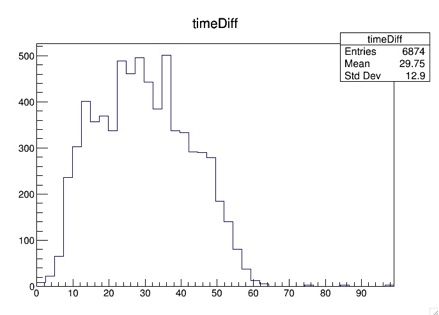
\includegraphics[height=95mm]{TimeDistSim.jpeg}}
	\caption[ Time Distribution of Simulation]{ The time distribution of simulation}
	\label{fig:TimeDiffSim}
\end{figure}
	
	Comparing the vertical positions and the radial positions for different cross talk probabilities found in Fig. \ref{fig:XtalkVerticalComp} and Fig.\ref{fig:XtalkRadialComp} respectively. Here black is 3\%, red is 5\%, green is 10\%, and Blue is 15\%.  These plots show that for a significant amount of data that the cross talk will not have a significant effect on the vertical or radial distributions.  However, I need to get a number for error associated with the cross-talk probability and we know it is not zero.  Furthermore, it is necessary to find out how many tracks are affected by the cross talk and specifically how the cross-talk effects the extrapolated vertical and radial positions.  \ref{fig:tracksXtalk} and shows the percentage of tracks with cross talk found in them vs. the cross talk probability. Here the y axis is in percentage of tracks which shows that only $0.5\%$ of the tracks make it past the track finding algorithm which shows how robust this algorithm is.  Fig.\ref{fig:YDiffXtalk} shows the difference between a track with and without cross talk for the vertical distribution. Using these numbers of the standard deviations and the means and the percentage of these tracks that are found in the final data gives an error of $<0.005 mm$.

\begin{figure}
	\centerline{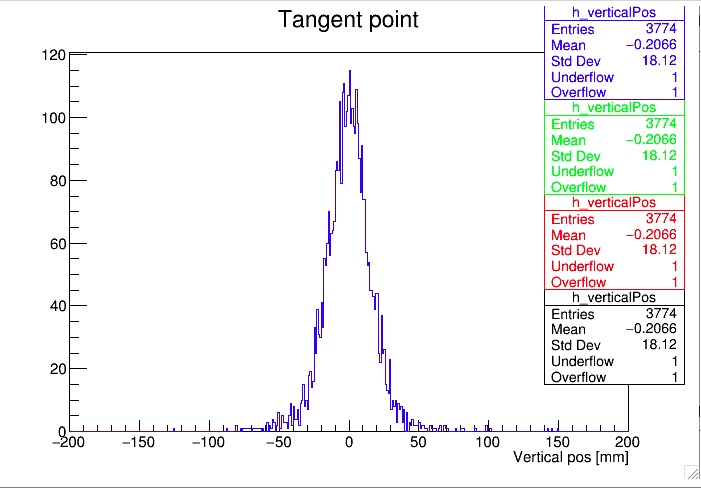
\includegraphics[height=95mm]{XtalkVerticalComp.jpeg}}
	\caption[ Comparison of the Vertical Distribution]{ Comparison of vertical Distribution with different amount of cross talk 3\% (black) 5\%(Red) 10\%(Green) 15\%(Blue)}
	\label{fig:XtalkVerticalComp}
\end{figure}



\begin{figure}
	\centerline{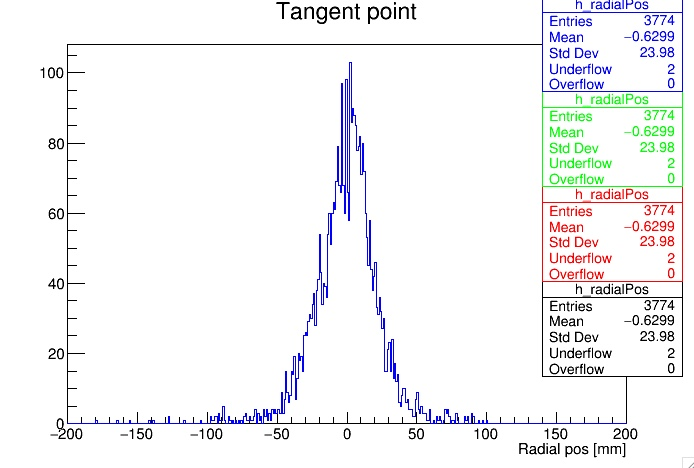
\includegraphics[height=95mm]{XtalkRadialComp.jpeg}}
	\caption[ Comparison of the Radial Distribution]{ Comparison of radial Distribution with different amount of cross talk 3\% (black) 5\%(Red) 10\%(Green) 15\%(Blue)}
	\label{fig:XtalkRadialComp}
\end{figure}


\begin{figure}
	\centerline{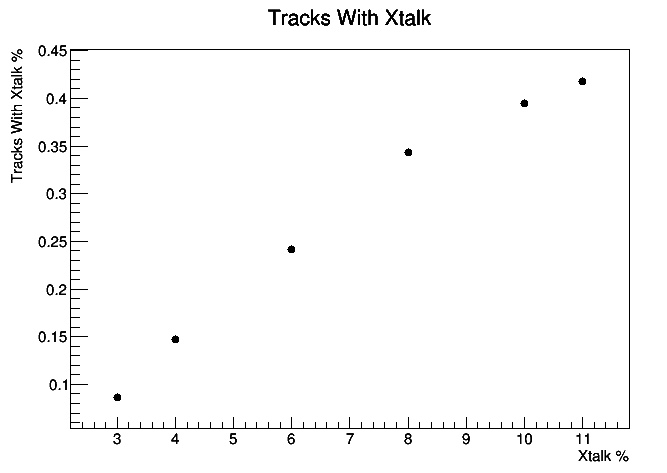
\includegraphics[height=95mm]{TracksXtalk.jpeg}}
	\caption[Tracks with Xtalk]{ Number of tracks with cross talk that are found anywhere in them}
	\label{fig:tracksXtalk}
\end{figure}


\begin{figure}
	\centerline{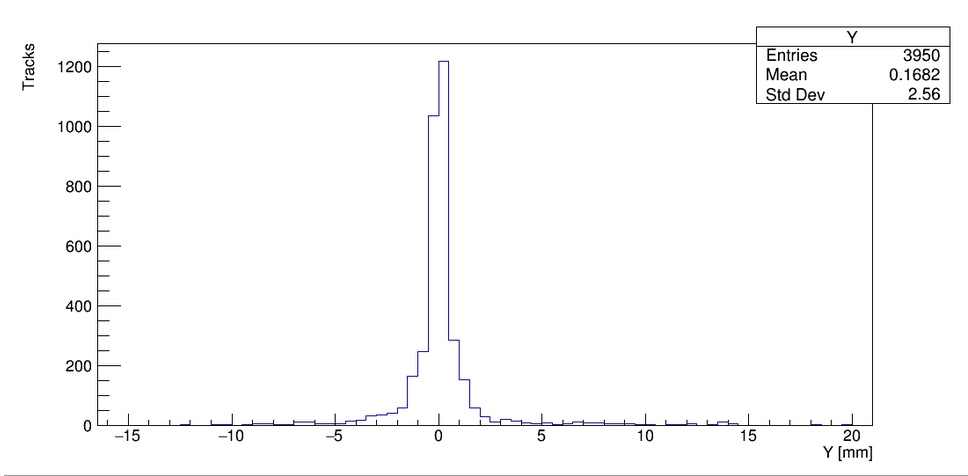
\includegraphics[height=95mm]{YDiffXtalk.jpeg}}
	\caption[Difference in Y with Xtalk]{ The Difference in Vertical positions in tracks with Cross Talk}
	\label{fig:YDiffXtalk}
\end{figure}




\section{Hit Resolution in the Straw Trackers}
	Hit resolution in the straw trackers is the spatial resolution at which we are able to determine the distance of closest approach to the wire in question from the found drift time of that hit. This is an important parameter since this establishes how well we are able to fit the track in the end.  The resolution can change throughout the course of data collection and therefore the properties of the resolution need to be established and the effect of the changes of the resolution need to be properly evaluated.

\subsection{General Explanation of Hit Resolution}

	The hit resolution in the straw trackers is determined from our ability to model the distance of closest approach to the corresponding drift times. The resolution is defined by the model of the radius to time determination of the straws, which is our modeled drift time vs the distance of closest approach. This model can change with different gasses, pressures temperatures of the surrounding environment. In addition, our model can change with variances in the voltage applied to the detectors.

\subsection{Evaluation of Changes in Hit Resolution}

To evaluate of time to radius distribution it is needed to find a way to observe and model the time to radius distribution in the straw tracker. To do this there was a method developed by James Mott \cite{jMottmiss} which was called the missing layers experiment. In the missing layers experiment there were a  particular selection of tracks, and then there was removed a particular layer from the tracking algorithm so that we can look at where the fitted track lands on a wire without having the fitting process effect the results. This would be the actual distance of closest approach, and then there was observed the corresponding drift times. Please refer to Fig. \ref{fig:Missing Layers} which gives a pictorial representation of the experiment.

\begin{figure}
	\centerline{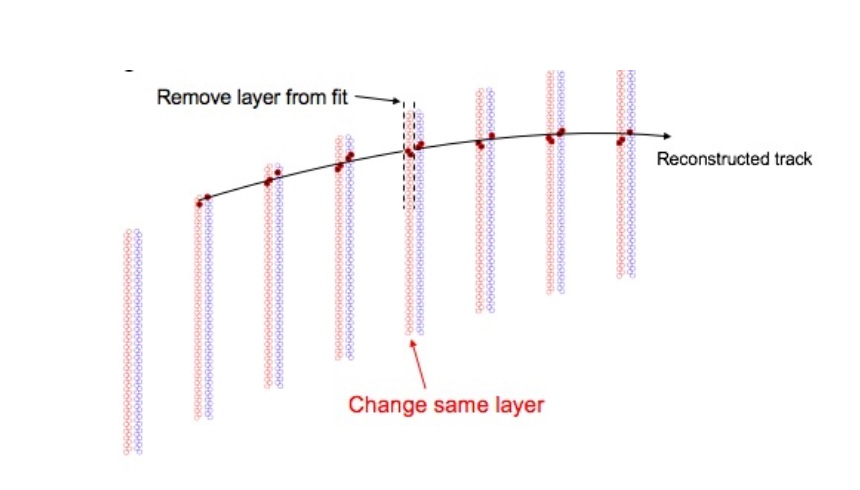
\includegraphics[height=95mm]{MissingLayers.jpeg}}
	\caption[Missing Layers]{ A pictorial representation of the missing layers experiment}
	\label{fig:Missing Layers}
\end{figure}

\begin{figure}
	\centerline{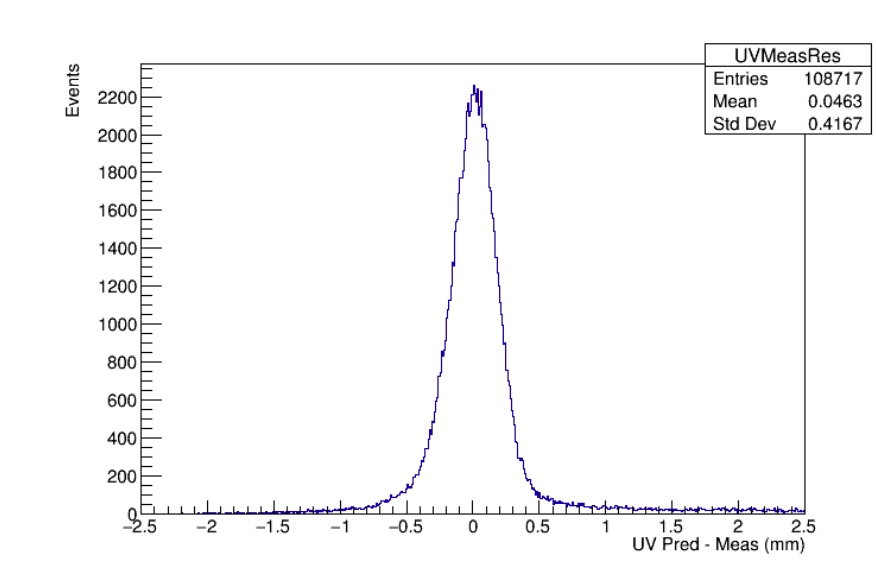
\includegraphics[height=95mm]{BadSpacialRes.jpeg}}
	\caption[Spacial Resolution with no track cuts]{ Resolution with no track cuts}
	\label{fig:badRes}
\end{figure}


	 If we look at this data with no particular tracks selections , found in Fig. \ref{fig:badRes} , we can see that there are tails associated with this semi-gaussian distribution. These tails make it difficult to fit the distribution and also skews our results for our characterization and it was necessary to look at these tracks that fall on the edge of the distribution as to improve our characterization and results. To do so we looked at a small subsection of these tracks with a plotting program that showed these tracks so that we could see what was going on. It was found that there were multiple different cases were the tracks were not properly representing the data that we wanted to look at. Firstly, corresponding to the previous section we have some cases were there might be cross talk or other similar effects, so here we required that is one digit per layer for each track so that we are not looking at the variances of cross talk. Secondly, to simplify the situation and to minimize the chance of error since there may be a lot of other things going on in the code, we required that for a particular time island that there is only one track going through the detectors at a time. By looking at the tracks we found a couple particular cases that happed pretty often.  One case it was found that a good portion of the tracks in the outliers were tracks that ended or began on the particular layer that we are studying. Here the track fitting with this missing layer caused the track fitting to not properly represent the true trajectory of the tracks and skewing our results. This was fixed by requiring that the tracks does not begin a couple of layers before and cannot end a couple of layers after the track. The next case that we found was tracks that there were extremely short tracks and they only hit a couple of layers. This causes the track fitting to be less precise due just to the shear number of data points given in the track. To evaluate how many digits that we needed the tracks to get rid of the tracks that are not being properly represented, we looked at the standard deviations of the resolution vs. the number of digits in the tracks found in Fig.\ref{fig:NumDigits},  Here you notice that we start to get a the large tails at when there is about 12 digits in the tracks, therefore we required that there are more than 12 digits in the track for this particular study.  Another common case of the outliers that we found was the case where the particle in the track reflected off of something at the layer that we were trying to study as found in Fig. \ref{fig:RefTrack}. Here this is a problem because before we removed the layer this track would normally fail, however when we removed that layer this causes the chi squared value does not deviate out of range causing the tracks to not fail. To take care of the majority of these tracks we just put a more stringent cut on where the track begins and ends further improving our results.
	
\begin{figure}
	\centerline{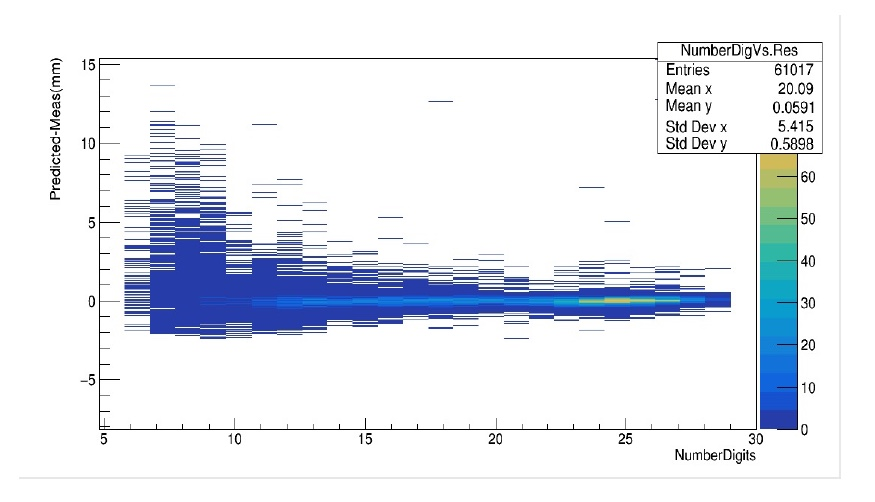
\includegraphics[height=95mm]{NumDigitsVsRes.jpeg}}
	\caption[Number of Digits vs. Resolution]{ The Number of digits associated with a track vs. the Resolution}
	\label{fig:NumDigits}
\end{figure} 

\begin{figure}
	\centerline{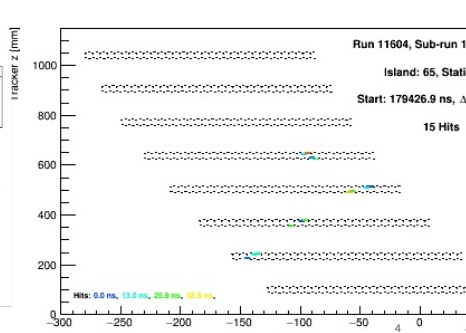
\includegraphics[height=95mm]{ReflectedTrack.jpeg}}
	\caption[Reflected Track]{ An example of a track being reflected off a boundary}
	\label{fig:RefTrack}
\end{figure} 

	 
	 
	 To show the effects of the previously established track selection I looked at what is called the distance of closest approach efficiency at the layer that was being studied. This will tell us how effectively we were able to predict the distance of closest approach which would show us if we had an improper track selection. To make this plot, first there was made a histogram of all the predicted distance of closest approach, as found in Fig. \ref{fig:dcaHits}, and there was made a histogram of the predicted track position minus the position of the wires in the layer, as found in Fig. \ref{fig:dcaTracks}. With the predicted distance of closest approach histogram is then divided by tracks positions histogram and normalized to the number of wires found in that layer. This will give what we call the distance of closest approach efficiency as found in Fig. {fig:badDCAeff}. This previous figure gives us our initial results before the tracks selection which establishes that if the tracks hits a particular straw in the layer, which is less than 3mm, it is seen that we are only predicting $90\%$  of our tracks. This result is definitely not correct since if a particle hits a straw we should be able to detect this. Now, If we look at Fig. \ref{fig:goodDCAeff} with our current tracks selection we can see similarly that we have a $99\%$ efficiency which is a more reasonable number and tells us that we are more effectively measuring the resolution. Now if we look at the resolution distribution before which is found in Fig. \ref{fig:badRes} and the resolutions distribution after, Fig. \ref{fig:goodRes}, with most of the tails of this distribution are now pretty much gone and the distribution looks more gaussian with a smaller standard deviation.


\begin{figure}
	\centerline{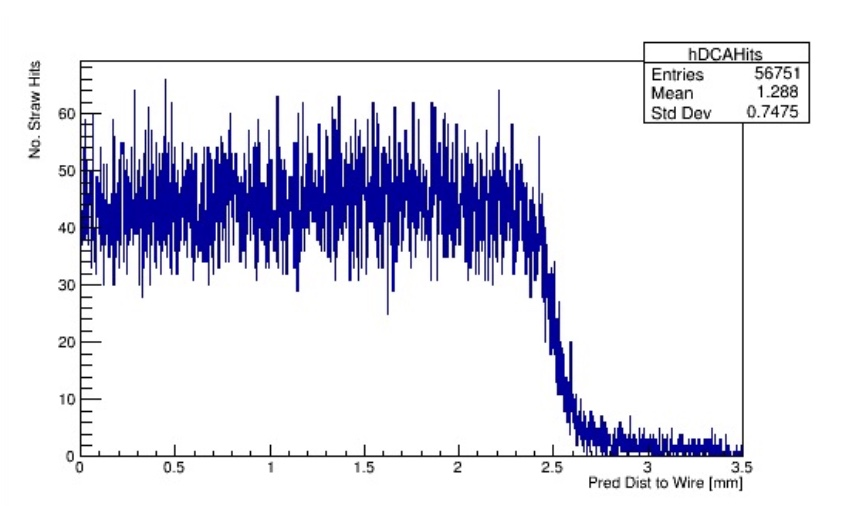
\includegraphics[height=95mm]{DCAHits.jpeg}}
	\caption[dcaHits]{ All the predicted DCA Hits}
	\label{fig:dcaHits}
\end{figure} 	

\begin{figure}
	\centerline{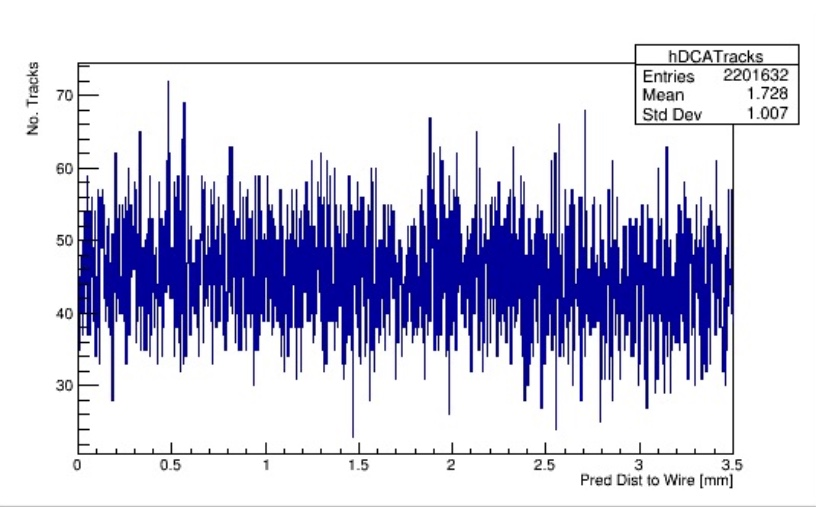
\includegraphics[height=95mm]{DCATracks.jpeg}}
	\caption[DCA Tracks]{ All the DCA's determined by the track postion}
	\label{fig:dcaTracks}
\end{figure} 

\begin{figure}
	\centerline{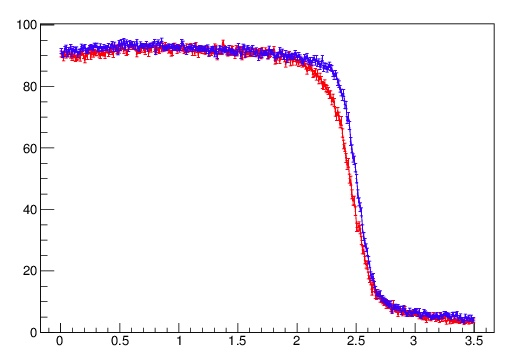
\includegraphics[height=95mm]{BadDCAEff.jpeg}}
	\caption[BadDCAEfficiency]{ The DCA Efficiency with poor track selection black is 1550V red is1660V}
	\label{fig:badDCAeff}
\end{figure} 	


\begin{figure}
	\centerline{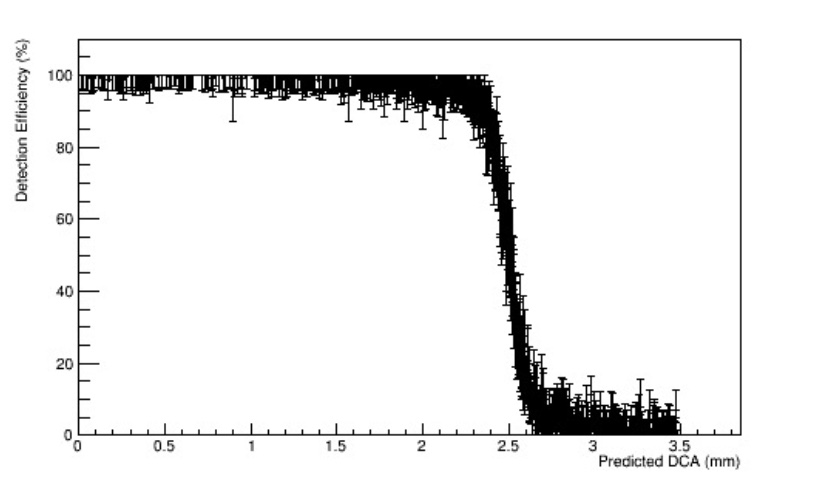
\includegraphics[height=95mm]{GoodDCAEff.jpeg}}
	\caption[Good DCA Effieciency]{ The DCA Effienciency}
	\label{fig:goodDCAeff}
\end{figure} 	

	 
	 Another thing to effectively measure the property of the resolution we needed to fit this function with an appropriate function. Although, this function looks fairly gaussian, which is what should happen when measuring the resolution, if we fit to a gaussian we can see we are not effectively fitting this histogram, found in Fig. \ref{fig:NoGoodRes}. This deviation in the histogram from being a true gaussian occurs because what is actually being measured is a couple of different resolutions occurring at the same time, we have the resolution of our track fitting algorithm and we have the resolution of our distance of closest approach model. In addition, we have the effects of the gas that we are using along with timing differences in the detectors...etc. Knowing this there is a motivation to fit this function to multiple gaussians, one fixed at the core and another one to broadly overly to take in account the tails in the distribution. In Fig.\ref{fig:goodRes}  is an example of the new fitting method which shows that we get a well established fitting function for the resolution plot. Then the overall distribution standard deviation by adding the standard deviations based on there mean in quadrature. Now that it is established the method to evaluate the resolution we now what causes deviations in the hit resolution.
	
	%% add in formula
	
\begin{figure}
	\centerline{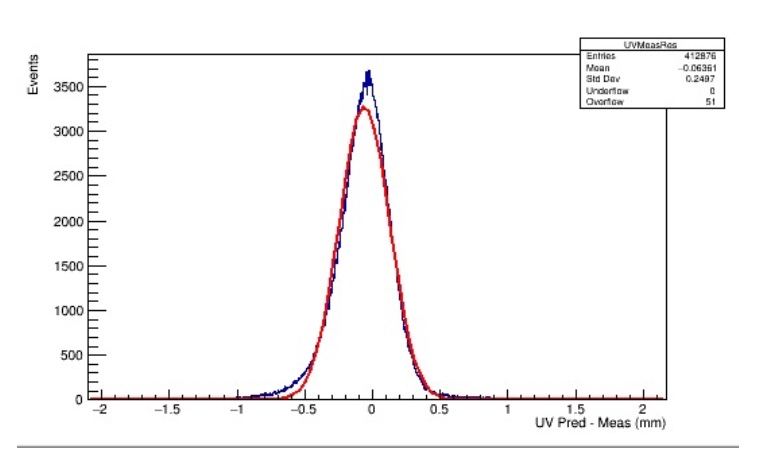
\includegraphics[height=95mm]{ResolutionNoGoodFit.jpeg}}
	\caption[Spacial Resolution with no track cuts]{ Resolution with poor fitting}
	\label{fig:NoGoodRes}
\end{figure}
	
\begin{figure}
	\centerline{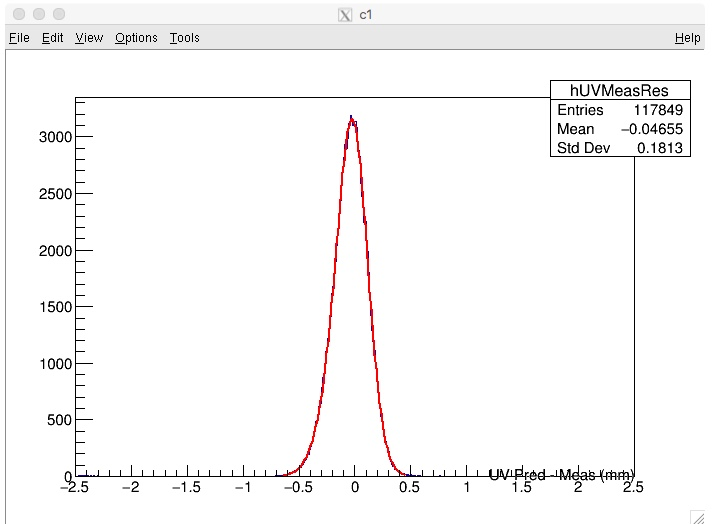
\includegraphics[height=95mm]{GoodRes.jpeg}}
	\caption[Good Resolution]{ Resolution with the proper track cuts and good fit}
	\label{fig:goodRes}
\end{figure} 		
	
	
	 
\subsection{Evaluation of Changes of Resolution}

	Using the methods establish in the previous section we now want to talk a look at how the resolution varies for changes in voltages, temperatures, pressures, and from run to run. This is important to understand how to model the changes in a simulation as to study how much of an effect this has on our data, and gives us information on how we can further improve the resolution of the detectors.
	
	The first study that was done was called the HV Scans experiment. Here when the beam was on there were tracks collected when we varied the voltage on the detector for the particular layers that we were studying, while keeping all the other detectors the same. Now this tells us how our model deviates vs.changes in voltages without ever affecting the track fitting process which gives us the effect that we are looking for.  Here we studied both stations (12, 18) and looked at the 3rd tracker in the first two layers from the direction of the beam which gives us a good example of tracks in the middle of the detector. In Fig.\ref{fig:ResVolt} it is seen that we definitely get a variance due to voltage changes which is expected however, we can see from the plot that we only get a variance of 0.04mm over the course of 160 Volts. This is a large voltage variation as compared to the variation that we would expect under normal conditions. Notice, that we get better resolution as we increase the voltage, this is due to the fact that as we get higher voltages we get larger deviations in the drift times and we are more able to pick out the distance of closest approach according to the model. In addition, notice that we also get fairly large deviations in the plot away from the linear relationship that this seems to follow, this follows from the fact that this data was collected over a period of 12 hours and there could be large deviations in all the other parameters that could effect the resolution, therefore these deviations are not out of line.

\begin{figure}
	\centerline{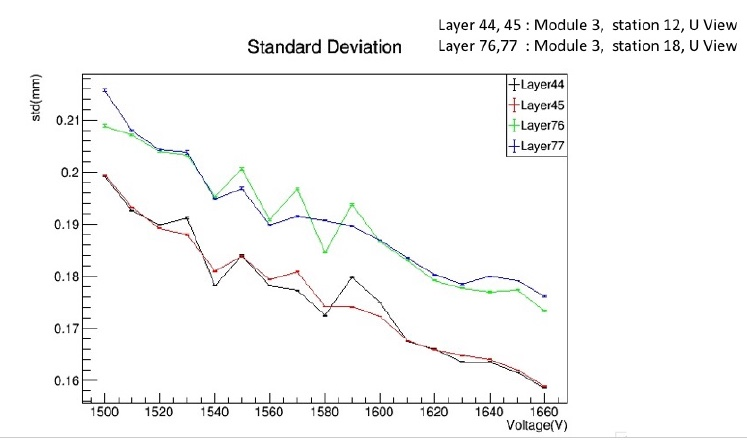
\includegraphics[height=95mm]{ResolutionVsVoltage.jpeg}}
	\caption[Resolution Vs Voltage]{ Resolution vs Voltage}
	\label{fig:ResVolt}
\end{figure} 	

	For the rest of the studies of the resolution it is necessary to have significant amount of data collected over a large period of time, here the what is called the 60 hour data set was used. As it sounds this was data that was collected with over a continuous 60 hour period. In Fig \ref{fig:ResNum} there is the resolution for layers 44, 45, 76 ,and 77 from run to run we can observe that there is roughly a $10\%$ deviation in the resolution over the course of the experiment. Here the error bars are given by the fitting errors established in the previous section. Furthermore, to investigate how much the resolution varies over the course of the run I took two runs and measured the resolution in subset of 10 sub-runs and looked at the resolution, this is found in Fig.\ref{fig:ResRun} which shows that there is approximately $13\%$ variance over the course of the run.
\begin{figure}
	\centerline{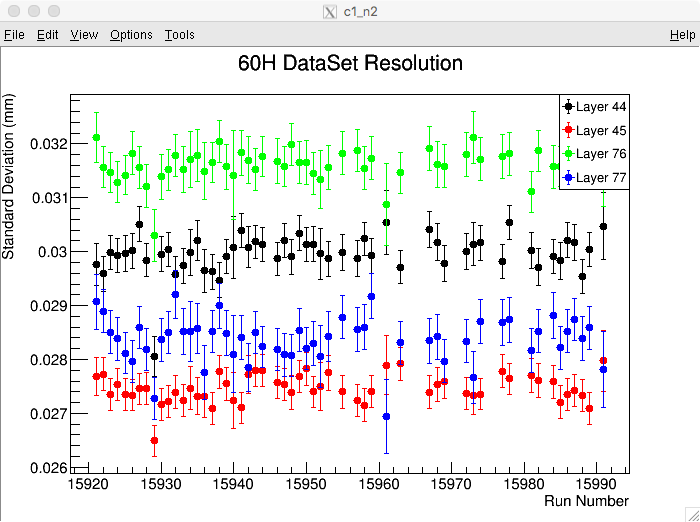
\includegraphics[height=95mm]{60HDataSetResidual.png}}
	\caption[60H Resolution]{ Resolution Vs. Run Number}
	\label{fig:ResNum}
\end{figure} 


\begin{figure}
	\centerline{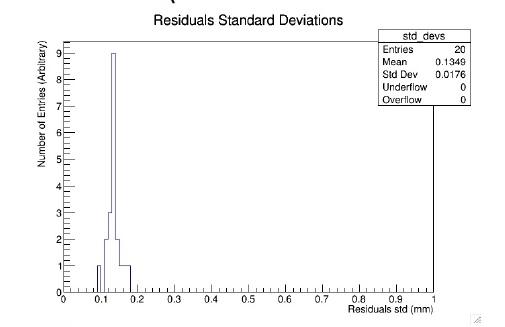
\includegraphics[height=95mm]{ResidualsRun.jpeg}}
	\caption[Resolution Over Two Runs]{ Resolution Over Two Runs}
	\label{fig:ResRun}
\end{figure} 


	
	 Now that we have this data we can look at the average pressures, temperatures, and humidity over the course of these runs. In Fig. \ref{{fig:TempRun}} is how the temperature in the experiment room varies over the course of data collection which we can see there is quite a large variance. Next, by looking at the average temperature over the course of a run vs. the resolutions from run by run , Fig. \ref{{fig:TempRun}}, we can see that there is no significant correlation between temperature and resolution changes with a Pearson correlation coefficient of 0.0643078. It was shown by another scholar that the track fitting changed with temperature by plotting the chi squared value vs. the temperature as shown in Fig. \ref{{fig:ChiRun}} which was expected to be from the resolution changes but it was shown that was not the case. To make sure this is the case it was investigated for my track selection that the chi squared values vs. temperature didn't change. Shown in Fig. \ref{fig:chiTemp} and Fig.  \ref{fig:chiRMS} shows the mean and standard deviations of the chi squared values do not vary with the temperature and have a small correlation factor. Therefore this reaffirmed by previous statement in saying the resolution was not significantly dependent on temperature in addition to saying that the deviation in the chi squared values vs. temperature was caused by something else that would bias the tracks.
	
\begin{figure}
	\centerline{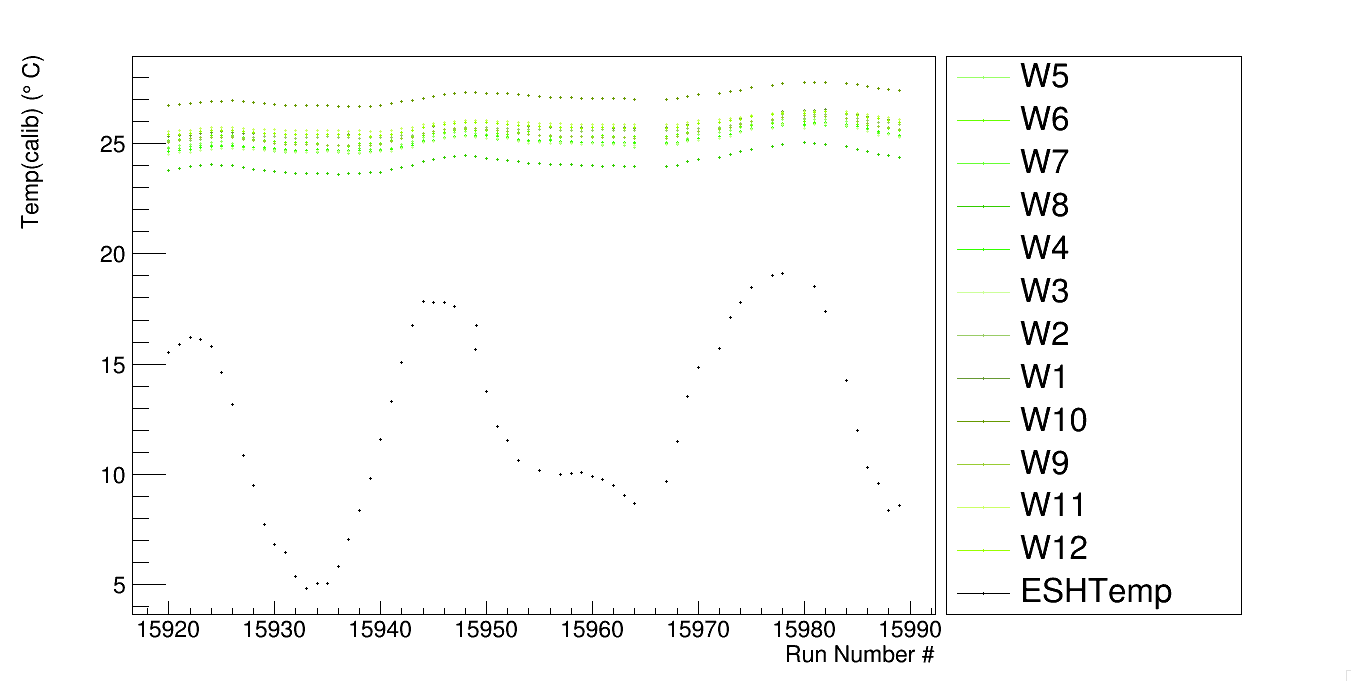
\includegraphics[height=95mm]{TempVsRunNumber.png}}
	\caption[Temperature Vs Run Number]{ Temperature Vs Run Number}
	\label{fig:TempRun}
\end{figure} 

\begin{figure}
	\centerline{\includegraphics[height=95mm]{VarianceVsTempIN.png}}
	\caption[Resolution Vs. Temperature]{Resolution Vs. Temperature}
	\label{fig:ResRun}
\end{figure} 

\begin{figure}
	\centerline{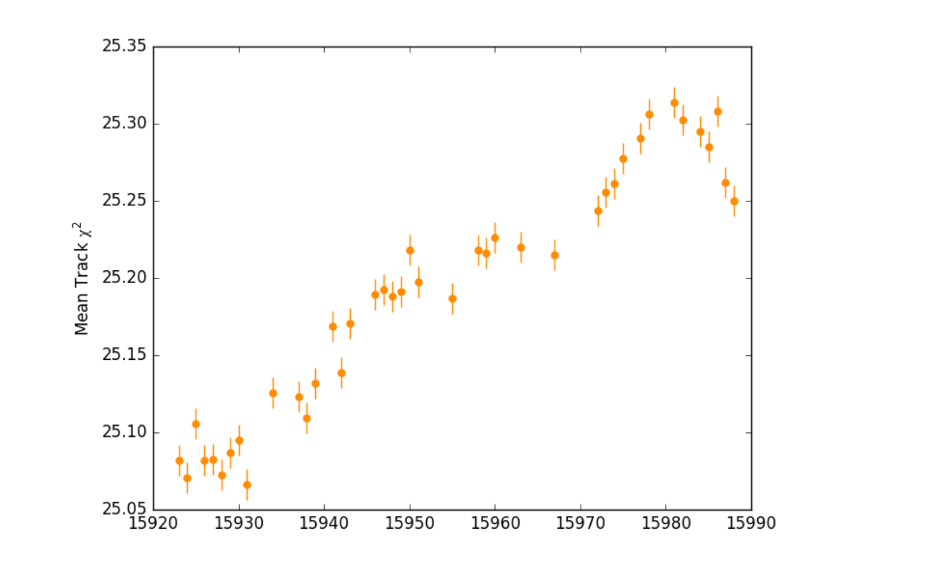
\includegraphics[height=95mm]{MeanChi260HDataSet.png}}
	\caption[Mean Chi2 over 60H Data Set]{ Mean Chi2 over 60H Data Set}
	\label{fig:ChiRun}
\end{figure} 

\begin{figure}
	\centerline{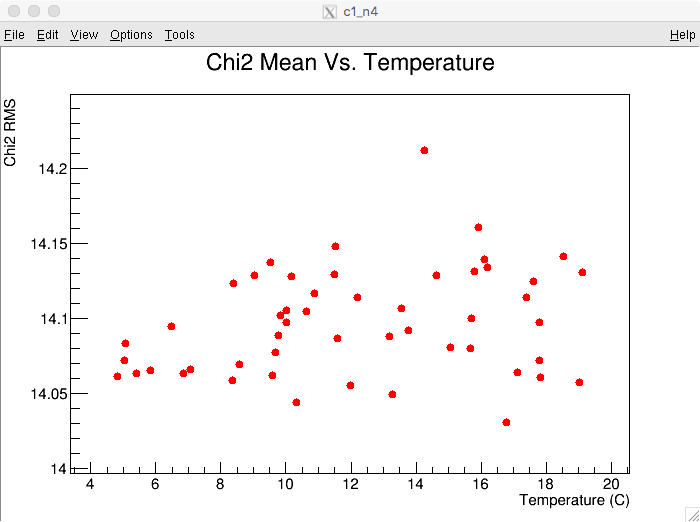
\includegraphics[height=95mm]{Chi2MeanVsTemp.png}}
	\caption[Chi2 Mean Vs. Temperature]{Chi2 Mean Vs. Temperature}
	\label{fig:chiTemp}
\end{figure} 
	 
\begin{figure}
	\centerline{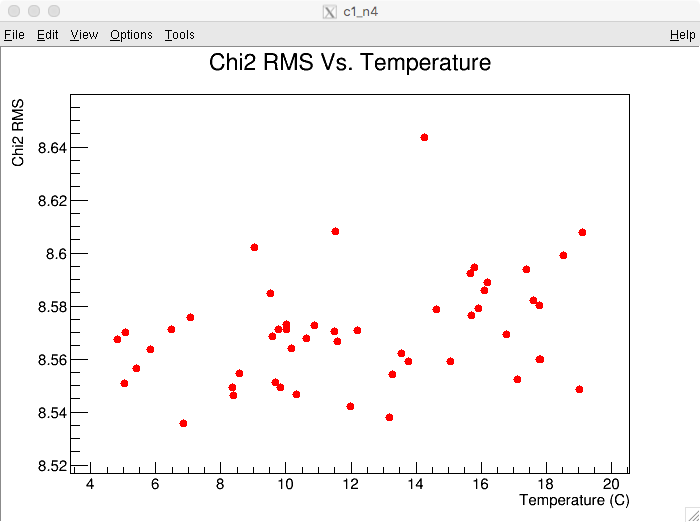
\includegraphics[height=95mm]{Chi2RMSVsTemp.png}}
	\caption[Chi2 RMS Vs. Temperature]{Chi2 RMS Vs. Temperature}
	\label{fig:chiRMS}
\end{figure} 	
	
		 
	 Next the correlation between pressures and resolutions were investigated in a similar way to the temperatures. In Fig. \ref {{fig:pressRun}}show how the pressure varied over the course of the runs that we are investigating. This shows that there is a changes of in pressure over the course of the collected data and this variation would show us if there were any changes of the resolution over normal pressure variances that we would see over the course of the experiment. Looking at the average pressure vs. resolution averaged from run to run, \ref {{fig:pressRun}}, again shows that there is no significant correlation between pressure and the resolution with no significant correlation factor.  Similarly, it was shown that the chi squared values varied vs. pressure again we wanted to make sure that this was not due to the resolution. Shown in Fig. ref{fig:chiMeanPres}and Fig. \ref{fig:chiRMSPres}shows the mean and standard deviations of the chi squared values do not vary and the variance is caused by some other changes in the tracks vs. pressure.
 \begin{figure}
	\centerline{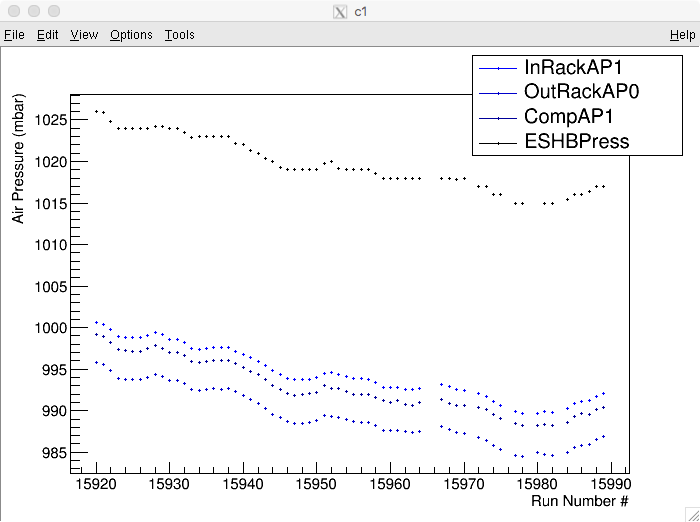
\includegraphics[height=95mm]{PressureVsRunNumber.png}}
	\caption[Pressure Vs Run Number]{Pressure Vs. Temperature}
	\label{fig:pressRun}
\end{figure} 	

\begin{figure}
	\centerline{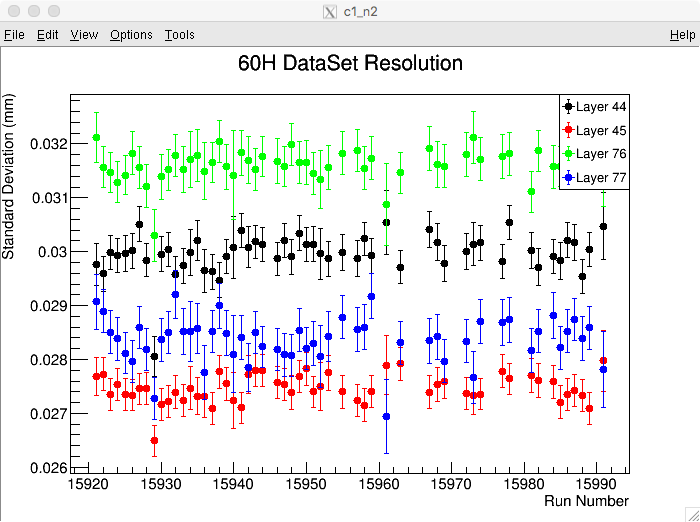
\includegraphics[height=95mm]{60HDataSetResidual.png}}
	\caption[Resolution Vs Run Number]{Resolution Vs. RunNumber}
	\label{fig:ResRun}
\end{figure} 


	
\begin{figure}
	\centerline{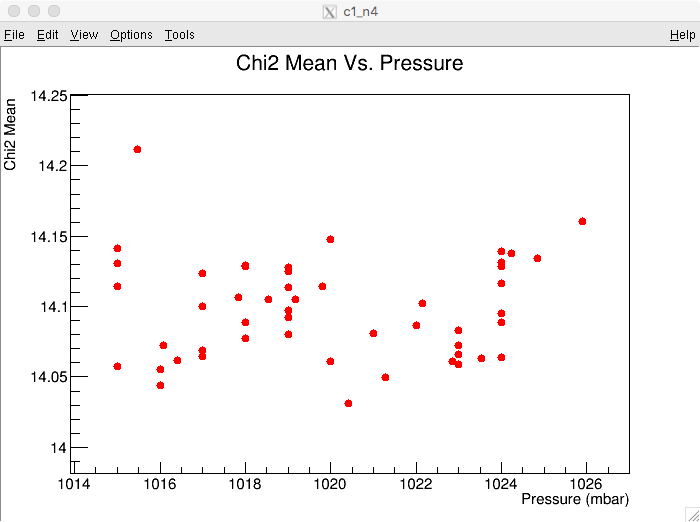
\includegraphics[height=95mm]{Chi2MeanVsPressure.png}}
	\caption[Chi2 Mean Vs. Pressure]{Chi2 Mean Vs. Pressure}
	\label{fig:chiMeanPres}
\end{figure}
	 
\begin{figure}
	\centerline{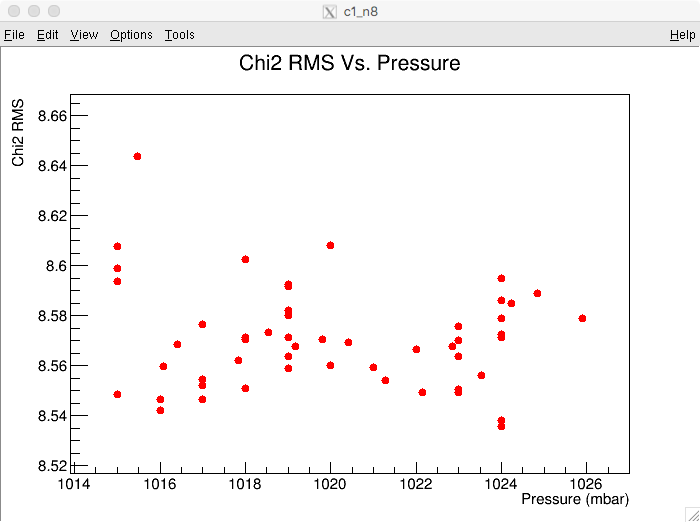
\includegraphics[height=95mm]{Chi2RMSVsPressure.png}}
	\caption[Chi2 RMS Vs. Pressure]{Chi2 RMS Vs. Pressure}
	\label{fig:chiRMSPres}
\end{figure}
	

	 
	 Now we have shown that for the effects that were established there is no significant effects on the resolution of the trackers. We also observed the amount that we would expect the tracker resolution to change over the course of the experiment which allows us to investigate how much of an effect this has on our final results.
	
\subsection{Changing Hit Resolution in Data}

		Now that we establish what causes changes and how much each effect causes changes in the hit resolution it is necessary to evaluate how much the changes affect our final results. To do so we took a look at one particular data set that has a given resolution value (This data was taken from one of the runs of the 60 hour data set) and randomly varied according to a gaussian distribution the distance of closest approach to some standard deviation value. This will give us the same effect as the resolution varying and we can look at how the extrapolation changes the vertical and radial distributions which is our main contribution to errors, as previously established. Practically, to do this experiment there was directly added in a section of code that randomly selects a value according to a gaussian distribution with a defined standard deviation and mean of zero. Then this randomly generated value was added to the distance of closest approach and passed this on to the rest of the code in the tracking algorithm. 
		
		Next we needed to see how much the radial and vertical position distributions are effected. In the previous section we showed that over the course of a run that there is a $13\%$ variance in resolution. Looking at the extrapolated y positions vs. different smearing percentages, Fig. \ref{{fig:AvgVertSmear}} , you can find that the average y position at $13\%$ only varies by a small amoun (Here the red line is at $13\%$) .  Even if we vary the resolution by $100\%$ the average y position changes by 3mm which is small compared to the other error contributions covered. Similarly, if we look at the standard deviation of the extrapolated vertical position vs smearing  Fig. \ref{fig:StdVertSmear}, we only see changes of 0.05mm at $13\%$ and 5mm at $100\%$ which also shows that this number is also not severely affected by the resolution changes by the numbers we have. Looking at the same plots except for the radial distribution we only, Fig. \ref{fig:AvgRadSmear} and Fig. \ref{fig:StdRadSmear}, we only observe 0.05mm of a change in the average radial position and 0.2mm change in radial standard deviation at the $13\%$  mark which again is a small contribution to the errors. 
\begin{figure}
	\centerline{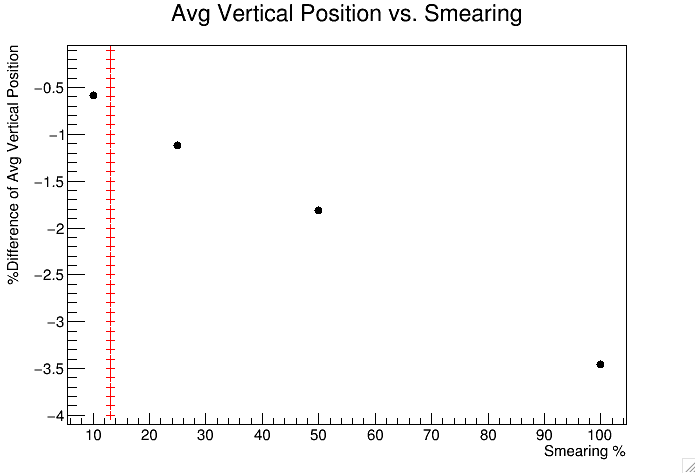
\includegraphics[height=95mm]{AvgVerticalSmear.png}}
	\caption[AvgVerticalSmear]{Difference in Vertical Position Vs. Smearing}
	\label{fig:AvgVertSmear}
\end{figure} 	

\begin{figure}
	\centerline{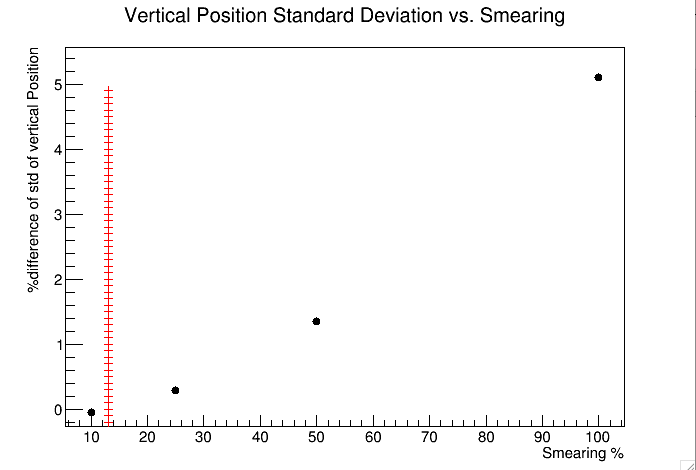
\includegraphics[height=95mm]{stdVerticalSmear.png}}
	\caption[stdVerticalSmear]{Difference in Vertical Position Standard Deviation Vs. Smearing}
	\label{fig:StdVertSmear}
\end{figure} 			
		
\begin{figure}
	\centerline{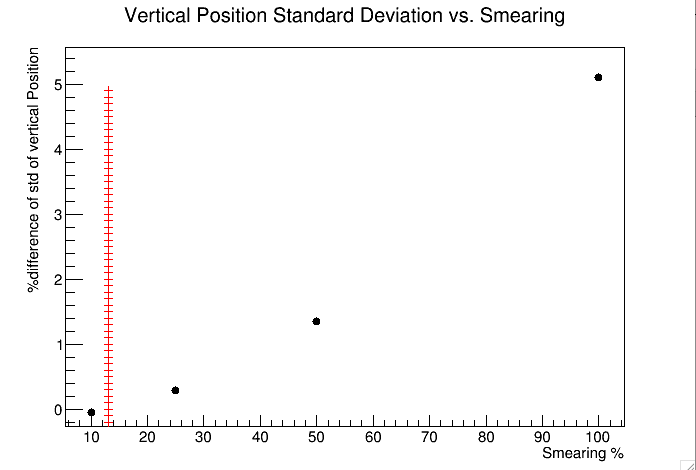
\includegraphics[height=95mm]{stdVerticalSmear.png}}
	\caption[stdVerticalSmear]{Difference in Vertical Position Standard Deviation Vs. Smearing}
	\label{fig:StdVertSmear}
\end{figure} 
	
\begin{figure}
	\centerline{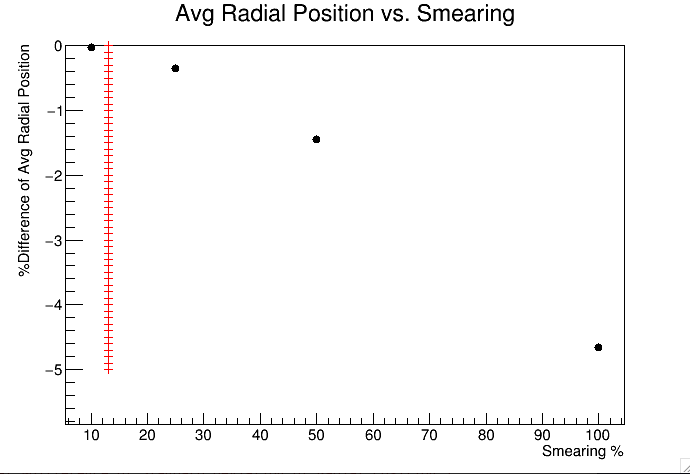
\includegraphics[height=95mm]{AvgRadialSmear.png}}
	\caption[AverageRadialSmear]{Difference in Radial PositionVs. Smearing}
	\label{fig:AvgRadSmear}
\end{figure} 

\begin{figure}
	\centerline{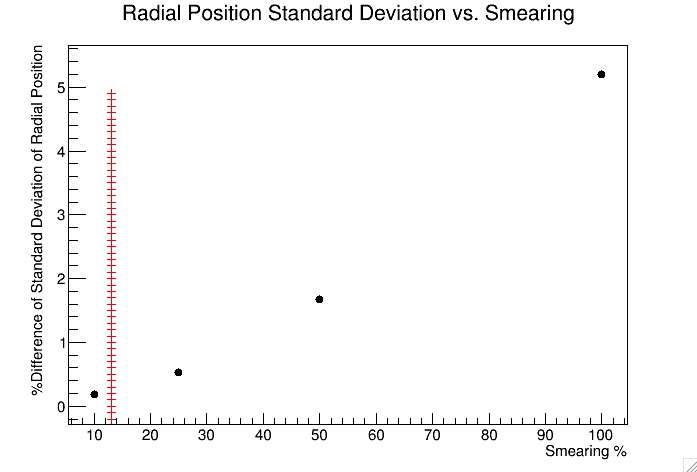
\includegraphics[height=95mm]{stdRadialSmear.png}}
	\caption[Standard DeviationRadialSmear]{Difference in Radial Position Standard Deviation Vs. Smearing}
	\label{fig:StdRadSmear}
\end{figure} 


\section{Results and Conclusions}

	In this chapter it has been explained the work that I have done towards trying to understand the systematics and there contributions to the final numbers. In other contributors work It has been found that with the current tracking algorithm that there are many corrections to the tracking algorithms that can be worked towards to improve the results of the EDM analysis. With the work that I have done I have shown that these two main effects that I have studied both the cross talk and the resolution of the detector contribute in a very small fashion. I showed that cross talk will only effect the final numbers to the $<$0.005ppb level in which the largest effects mainly the tracker alignment contribute to the 0.3 ppblevel. In addition, I have found that due to the resolution changes that we would expect over the course of the experiment and is also small and it effects the final measurement to the 0.03 ppb level. In conclusion, it has been found that there are other areas in the tracking which would contribute more than these errors.


\end{document}